\documentclass[1p]{elsarticle_modified}
%\bibliographystyle{elsarticle-num}

%\usepackage[colorlinks]{hyperref}
%\usepackage{abbrmath_seonhwa} %\Abb, \Ascr, \Acal ,\Abf, \Afrak
\usepackage{amsfonts}
\usepackage{amssymb}
\usepackage{amsmath}
\usepackage{amsthm}
\usepackage{scalefnt}
\usepackage{amsbsy}
\usepackage{kotex}
\usepackage{caption}
\usepackage{subfig}
\usepackage{color}
\usepackage{graphicx}
\usepackage{xcolor} %% white, black, red, green, blue, cyan, magenta, yellow
\usepackage{float}
\usepackage{setspace}
\usepackage{hyperref}

\usepackage{tikz}
\usetikzlibrary{arrows}

\usepackage{multirow}
\usepackage{array} % fixed length table
\usepackage{hhline}

%%%%%%%%%%%%%%%%%%%%%
\makeatletter
\renewcommand*\env@matrix[1][\arraystretch]{%
	\edef\arraystretch{#1}%
	\hskip -\arraycolsep
	\let\@ifnextchar\new@ifnextchar
	\array{*\c@MaxMatrixCols c}}
\makeatother %https://tex.stackexchange.com/questions/14071/how-can-i-increase-the-line-spacing-in-a-matrix
%%%%%%%%%%%%%%%

\usepackage[normalem]{ulem}

\newcommand{\msout}[1]{\ifmmode\text{\sout{\ensuremath{#1}}}\else\sout{#1}\fi}
%SOURCE: \msout is \stkout macro in https://tex.stackexchange.com/questions/20609/strikeout-in-math-mode

\newcommand{\cancel}[1]{
	\ifmmode
	{\color{red}\msout{#1}}
	\else
	{\color{red}\sout{#1}}
	\fi
}

\newcommand{\add}[1]{
	{\color{blue}\uwave{#1}}
}

\newcommand{\replace}[2]{
	\ifmmode
	{\color{red}\msout{#1}}{\color{blue}\uwave{#2}}
	\else
	{\color{red}\sout{#1}}{\color{blue}\uwave{#2}}
	\fi
}

\newcommand{\Sol}{\mathcal{S}} %segment
\newcommand{\D}{D} %diagram
\newcommand{\A}{\mathcal{A}} %arc


%%%%%%%%%%%%%%%%%%%%%%%%%%%%%5 test

\def\sl{\operatorname{\textup{SL}}(2,\Cbb)}
\def\psl{\operatorname{\textup{PSL}}(2,\Cbb)}
\def\quan{\mkern 1mu \triangleright \mkern 1mu}

\theoremstyle{definition}
\newtheorem{thm}{Theorem}[section]
\newtheorem{prop}[thm]{Proposition}
\newtheorem{lem}[thm]{Lemma}
\newtheorem{ques}[thm]{Question}
\newtheorem{cor}[thm]{Corollary}
\newtheorem{defn}[thm]{Definition}
\newtheorem{exam}[thm]{Example}
\newtheorem{rmk}[thm]{Remark}
\newtheorem{alg}[thm]{Algorithm}

\newcommand{\I}{\sqrt{-1}}
\begin{document}

%\begin{frontmatter}
%
%\title{Boundary parabolic representations of knots up to 8 crossings}
%
%%% Group authors per affiliation:
%\author{Yunhi Cho} 
%\address{Department of Mathematics, University of Seoul, Seoul, Korea}
%\ead{yhcho@uos.ac.kr}
%
%
%\author{Seonhwa Kim} %\fnref{s_kim}}
%\address{Center for Geometry and Physics, Institute for Basic Science, Pohang, 37673, Korea}
%\ead{ryeona17@ibs.re.kr}
%
%\author{Hyuk Kim}
%\address{Department of Mathematical Sciences, Seoul National University, Seoul 08826, Korea}
%\ead{hyukkim@snu.ac.kr}
%
%\author{Seokbeom Yoon}
%\address{Department of Mathematical Sciences, Seoul National University, Seoul, 08826,  Korea}
%\ead{sbyoon15@snu.ac.kr}
%
%\begin{abstract}
%We find all boundary parabolic representation of knots up to 8 crossings.
%
%\end{abstract}
%\begin{keyword}
%    \MSC[2010] 57M25 
%\end{keyword}
%
%\end{frontmatter}

%\linenumbers
%\tableofcontents
%
\newcommand\colored[1]{\textcolor{white}{\rule[-0.35ex]{0.8em}{1.4ex}}\kern-0.8em\color{red} #1}%
%\newcommand\colored[1]{\textcolor{white}{ #1}\kern-2.17ex	\textcolor{white}{ #1}\kern-1.81ex	\textcolor{white}{ #1}\kern-2.15ex\color{red}#1	}

{\Large $\underline{11a_{257}~(K11a_{257})}$}

\setlength{\tabcolsep}{10pt}
\renewcommand{\arraystretch}{1.6}
\vspace{1cm}\begin{tabular}{m{100pt}>{\centering\arraybackslash}m{274pt}}
\multirow{5}{120pt}{
	\centering
	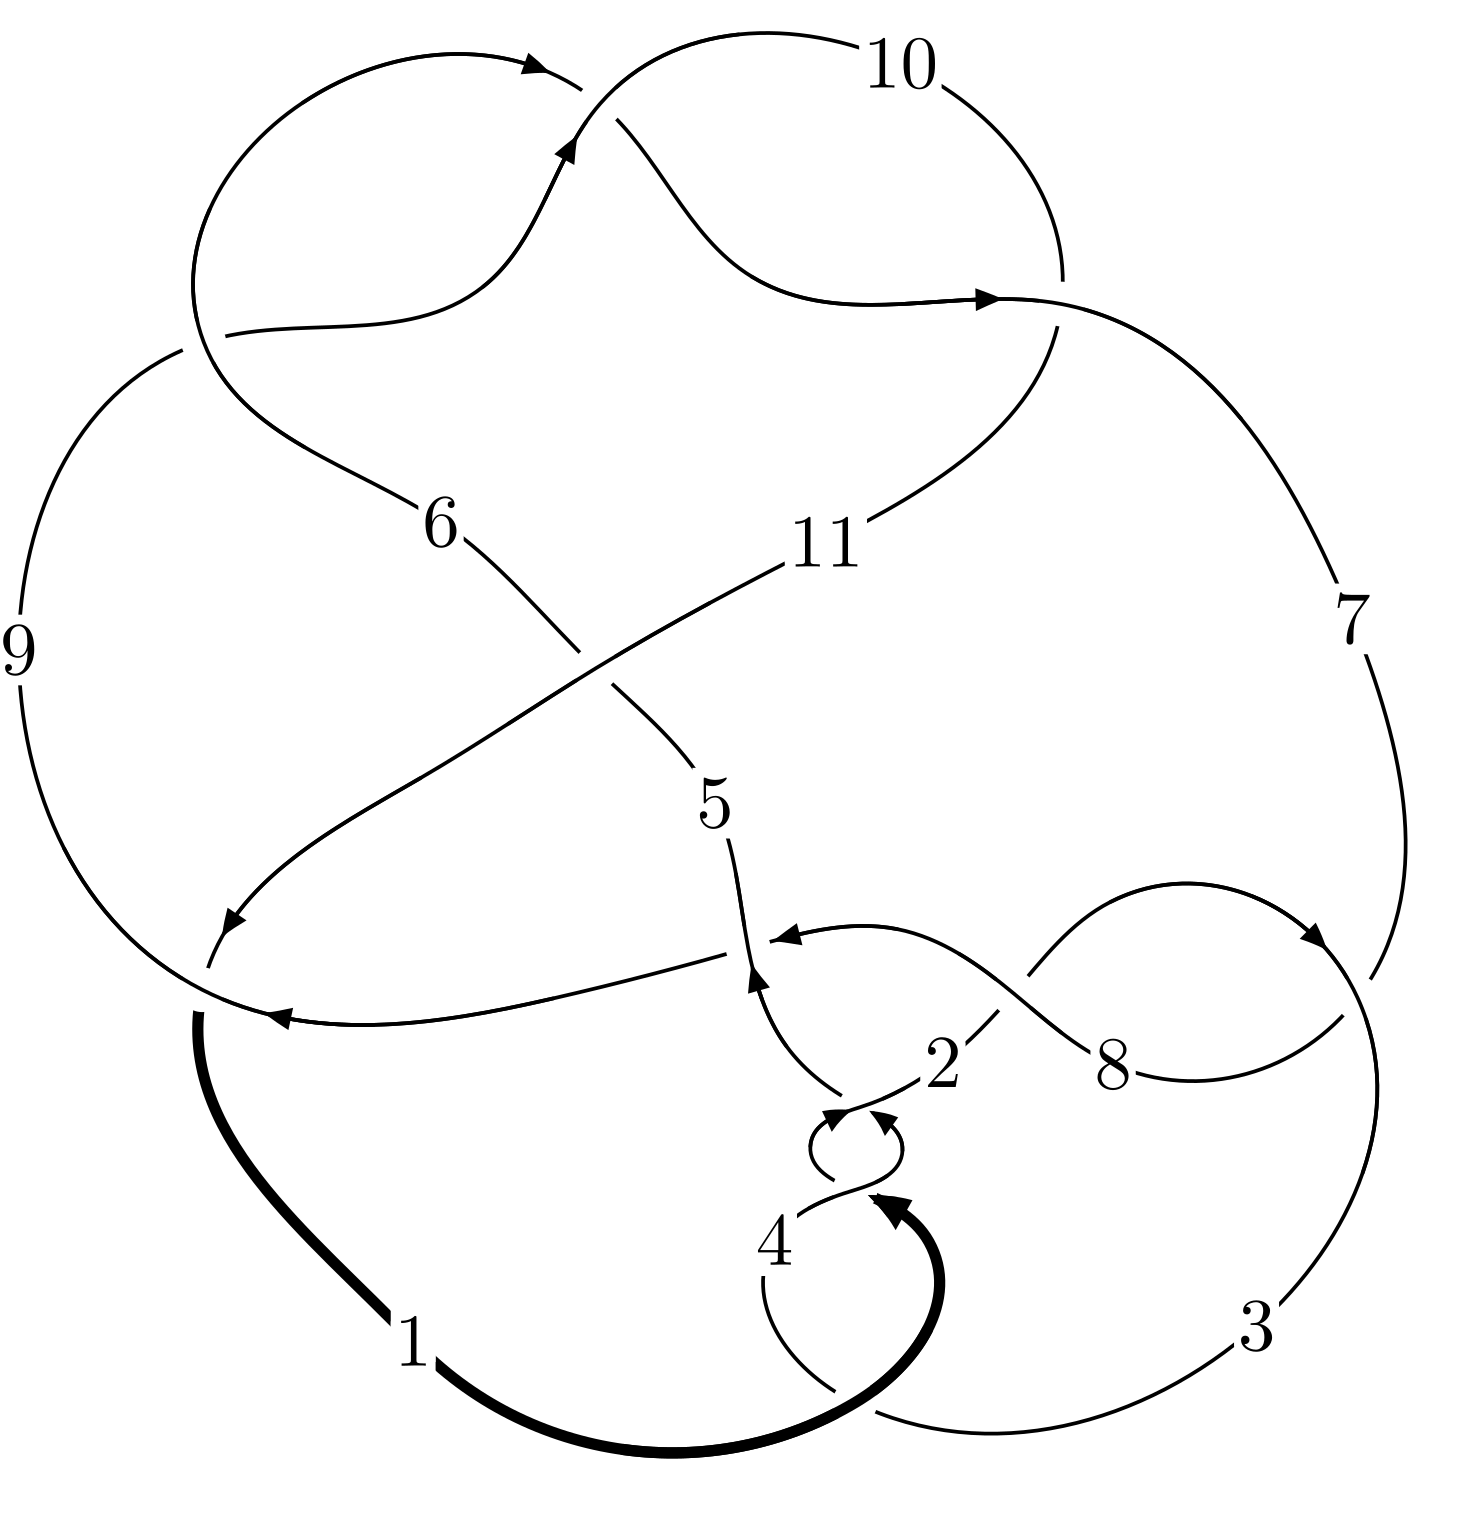
\includegraphics[width=112pt]{../../../GIT/diagram.site/Diagrams/png/506_11a_257.png}\\
\ \ \ A knot diagram\footnotemark}&
\allowdisplaybreaks
\textbf{Linearized knot diagam} \\
\cline{2-2}
 &
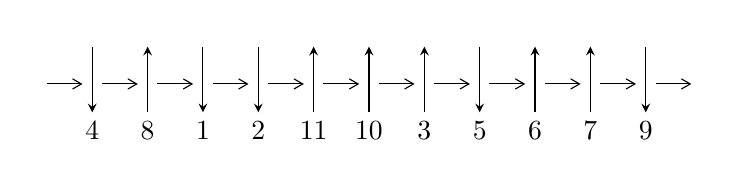
\begin{tikzpicture}[x=20pt, y=17pt]
	% nodes
	\node (C0) at (0, 0) {};
	\node (C1) at (1, 0) {};
	\node (C1U) at (1, +1) {};
	\node (C1D) at (1, -1) {4};

	\node (C2) at (2, 0) {};
	\node (C2U) at (2, +1) {};
	\node (C2D) at (2, -1) {8};

	\node (C3) at (3, 0) {};
	\node (C3U) at (3, +1) {};
	\node (C3D) at (3, -1) {1};

	\node (C4) at (4, 0) {};
	\node (C4U) at (4, +1) {};
	\node (C4D) at (4, -1) {2};

	\node (C5) at (5, 0) {};
	\node (C5U) at (5, +1) {};
	\node (C5D) at (5, -1) {11};

	\node (C6) at (6, 0) {};
	\node (C6U) at (6, +1) {};
	\node (C6D) at (6, -1) {10};

	\node (C7) at (7, 0) {};
	\node (C7U) at (7, +1) {};
	\node (C7D) at (7, -1) {3};

	\node (C8) at (8, 0) {};
	\node (C8U) at (8, +1) {};
	\node (C8D) at (8, -1) {5};

	\node (C9) at (9, 0) {};
	\node (C9U) at (9, +1) {};
	\node (C9D) at (9, -1) {6};

	\node (C10) at (10, 0) {};
	\node (C10U) at (10, +1) {};
	\node (C10D) at (10, -1) {7};

	\node (C11) at (11, 0) {};
	\node (C11U) at (11, +1) {};
	\node (C11D) at (11, -1) {9};
	\node (C12) at (12, 0) {};

	% arrows
	\draw[->,>={angle 60}]
	(C0) edge (C1) (C1) edge (C2) (C2) edge (C3) (C3) edge (C4) (C4) edge (C5) (C5) edge (C6) (C6) edge (C7) (C7) edge (C8) (C8) edge (C9) (C9) edge (C10) (C10) edge (C11) (C11) edge (C12) ;	\draw[->,>=stealth]
	(C1U) edge (C1D) (C2D) edge (C2U) (C3U) edge (C3D) (C4U) edge (C4D) (C5D) edge (C5U) (C6D) edge (C6U) (C7D) edge (C7U) (C8U) edge (C8D) (C9D) edge (C9U) (C10D) edge (C10U) (C11U) edge (C11D) ;
	\end{tikzpicture} \\
\hhline{~~} \\& 
\textbf{Solving Sequence} \\ \cline{2-2} 
 &
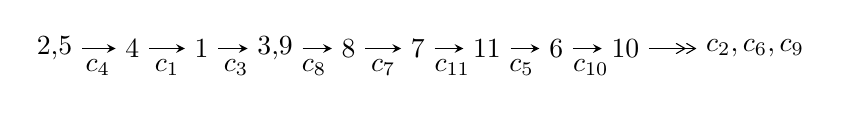
\begin{tikzpicture}[x=25pt, y=7pt]
	% node
	\node (A0) at (-1/8, 0) {2,5};
	\node (A1) at (1, 0) {4};
	\node (A2) at (2, 0) {1};
	\node (A3) at (49/16, 0) {3,9};
	\node (A4) at (33/8, 0) {8};
	\node (A5) at (41/8, 0) {7};
	\node (A6) at (49/8, 0) {11};
	\node (A7) at (57/8, 0) {6};
	\node (A8) at (65/8, 0) {10};
	\node (C1) at (1/2, -1) {$c_{4}$};
	\node (C2) at (3/2, -1) {$c_{1}$};
	\node (C3) at (5/2, -1) {$c_{3}$};
	\node (C4) at (29/8, -1) {$c_{8}$};
	\node (C5) at (37/8, -1) {$c_{7}$};
	\node (C6) at (45/8, -1) {$c_{11}$};
	\node (C7) at (53/8, -1) {$c_{5}$};
	\node (C8) at (61/8, -1) {$c_{10}$};
	\node (A9) at (10, 0) {$c_{2},c_{6},c_{9}$};

	% edge
	\draw[->,>=stealth]	
	(A0) edge (A1) (A1) edge (A2) (A2) edge (A3) (A3) edge (A4) (A4) edge (A5) (A5) edge (A6) (A6) edge (A7) (A7) edge (A8) ;
	\draw[->>,>={angle 60}]	
	(A8) edge (A9);
\end{tikzpicture} \\ 

\end{tabular} \\

\footnotetext{
The image of knot diagram is generated by the software ``\textbf{Draw programme}" developed by Andrew Bartholomew(\url{http://www.layer8.co.uk/maths/draw/index.htm\#Running-draw}), where we modified some parts for our purpose(\url{https://github.com/CATsTAILs/LinksPainter}).
}\phantom \\ \newline 
\centering \textbf{Ideals for irreducible components\footnotemark of $X_{\text{par}}$} 
 
\begin{align*}
I^u_{1}&=\langle 
178 u^{52}-830 u^{51}+\cdots+4 b+135,\;-82 u^{52}+389 u^{51}+\cdots+4 a-64,\;u^{53}-6 u^{52}+\cdots+5 u-1\rangle \\
I^u_{2}&=\langle 
b+a,\;a^5- a^4+2 a^3- a^2+a-1,\;u+1\rangle \\
\\
\end{align*}
\raggedright * 2 irreducible components of $\dim_{\mathbb{C}}=0$, with total 58 representations.\\
\footnotetext{All coefficients of polynomials are rational numbers. But the coefficients are sometimes approximated in decimal forms when there is not enough margin.}
\newpage
\renewcommand{\arraystretch}{1}
\centering \section*{I. $I^u_{1}= \langle 178 u^{52}-830 u^{51}+\cdots+4 b+135,\;-82 u^{52}+389 u^{51}+\cdots+4 a-64,\;u^{53}-6 u^{52}+\cdots+5 u-1 \rangle$}
\flushleft \textbf{(i) Arc colorings}\\
\begin{tabular}{m{7pt} m{180pt} m{7pt} m{180pt} }
\flushright $a_{2}=$&$\begin{pmatrix}0\\u\end{pmatrix}$ \\
\flushright $a_{5}=$&$\begin{pmatrix}1\\0\end{pmatrix}$ \\
\flushright $a_{4}=$&$\begin{pmatrix}1\\- u^2\end{pmatrix}$ \\
\flushright $a_{1}=$&$\begin{pmatrix}u\\- u^3+u\end{pmatrix}$ \\
\flushright $a_{3}=$&$\begin{pmatrix}- u^2+1\\u^4-2 u^2\end{pmatrix}$ \\
\flushright $a_{9}=$&$\begin{pmatrix}\frac{41}{2} u^{52}-\frac{389}{4} u^{51}+\cdots-\frac{285}{4} u+16\\-\frac{89}{2} u^{52}+\frac{415}{2} u^{51}+\cdots+143 u-\frac{135}{4}\end{pmatrix}$ \\
\flushright $a_{8}=$&$\begin{pmatrix}-24 u^{52}+\frac{441}{4} u^{51}+\cdots+\frac{287}{4} u-\frac{71}{4}\\-\frac{89}{2} u^{52}+\frac{415}{2} u^{51}+\cdots+143 u-\frac{135}{4}\end{pmatrix}$ \\
\flushright $a_{7}=$&$\begin{pmatrix}8 u^{52}-\frac{143}{4} u^{51}+\cdots-\frac{109}{4} u+\frac{21}{4}\\-\frac{183}{4} u^{52}+210 u^{51}+\cdots+\frac{559}{4} u-\frac{131}{4}\end{pmatrix}$ \\
\flushright $a_{11}=$&$\begin{pmatrix}\frac{1}{16} u^{52}-\frac{5}{16} u^{51}+\cdots+\frac{15}{4} u+\frac{17}{16}\\-\frac{1}{16} u^{52}+\frac{5}{16} u^{51}+\cdots+\frac{1}{4} u-\frac{1}{16}\end{pmatrix}$ \\
\flushright $a_{6}=$&$\begin{pmatrix}-0.937500 u^{52}+4.56250 u^{51}+\cdots+3.37500 u+0.187500\\\frac{9}{8} u^{52}-\frac{11}{2} u^{51}+\cdots-\frac{33}{8} u+1\end{pmatrix}$ \\
\flushright $a_{10}=$&$\begin{pmatrix}-\frac{1}{16} u^{52}+\frac{5}{16} u^{51}+\cdots+\frac{5}{4} u-\frac{1}{16}\\- u^{52}+\frac{39}{8} u^{51}+\cdots+\frac{37}{8} u-\frac{7}{8}\end{pmatrix}$\\ \flushright $a_{10}=$&$\begin{pmatrix}-\frac{1}{16} u^{52}+\frac{5}{16} u^{51}+\cdots+\frac{5}{4} u-\frac{1}{16}\\- u^{52}+\frac{39}{8} u^{51}+\cdots+\frac{37}{8} u-\frac{7}{8}\end{pmatrix}$\\&\end{tabular}
\flushleft \textbf{(ii) Obstruction class $= -1$}\\~\\
\flushleft \textbf{(iii) Cusp Shapes $= 95 u^{52}-\frac{3551}{8} u^{51}+\cdots-\frac{2445}{8} u+\frac{625}{8}$}\\~\\
\newpage\renewcommand{\arraystretch}{1}
\flushleft \textbf{(iv) u-Polynomials at the component}\newline \\
\begin{tabular}{m{50pt}|m{274pt}}
Crossings & \hspace{64pt}u-Polynomials at each crossing \\
\hline $$\begin{aligned}c_{1},c_{3},c_{4}\end{aligned}$$&$\begin{aligned}
&u^{53}-6 u^{52}+\cdots+5 u-1
\end{aligned}$\\
\hline $$\begin{aligned}c_{2},c_{7}\end{aligned}$$&$\begin{aligned}
&u^{53}+u^{52}+\cdots+32 u-32
\end{aligned}$\\
\hline $$\begin{aligned}c_{5}\end{aligned}$$&$\begin{aligned}
&u^{53}+6 u^{52}+\cdots+5 u+1
\end{aligned}$\\
\hline $$\begin{aligned}c_{6},c_{9},c_{10}\end{aligned}$$&$\begin{aligned}
&u^{53}-2 u^{52}+\cdots- u-1
\end{aligned}$\\
\hline $$\begin{aligned}c_{8}\end{aligned}$$&$\begin{aligned}
&u^{53}+2 u^{52}+\cdots-353 u-505
\end{aligned}$\\
\hline $$\begin{aligned}c_{11}\end{aligned}$$&$\begin{aligned}
&u^{53}-12 u^{52}+\cdots+577 u-73
\end{aligned}$\\
\hline
\end{tabular}\\~\\
\newpage\renewcommand{\arraystretch}{1}
\flushleft \textbf{(v) Riley Polynomials at the component}\newline \\
\begin{tabular}{m{50pt}|m{274pt}}
Crossings & \hspace{64pt}Riley Polynomials at each crossing \\
\hline $$\begin{aligned}c_{1},c_{3},c_{4}\end{aligned}$$&$\begin{aligned}
&y^{53}-52 y^{52}+\cdots-3 y-1
\end{aligned}$\\
\hline $$\begin{aligned}c_{2},c_{7}\end{aligned}$$&$\begin{aligned}
&y^{53}+33 y^{52}+\cdots-3584 y-1024
\end{aligned}$\\
\hline $$\begin{aligned}c_{5}\end{aligned}$$&$\begin{aligned}
&y^{53}+54 y^{51}+\cdots+3 y-1
\end{aligned}$\\
\hline $$\begin{aligned}c_{6},c_{9},c_{10}\end{aligned}$$&$\begin{aligned}
&y^{53}-48 y^{52}+\cdots-5 y-1
\end{aligned}$\\
\hline $$\begin{aligned}c_{8}\end{aligned}$$&$\begin{aligned}
&y^{53}-24 y^{52}+\cdots-2730661 y-255025
\end{aligned}$\\
\hline $$\begin{aligned}c_{11}\end{aligned}$$&$\begin{aligned}
&y^{53}+12 y^{52}+\cdots-67257 y-5329
\end{aligned}$\\
\hline
\end{tabular}\\~\\
\newpage\flushleft \textbf{(vi) Complex Volumes and Cusp Shapes}
$$\begin{array}{c|c|c}  
\text{Solutions to }I^u_{1}& \I (\text{vol} + \sqrt{-1}CS) & \text{Cusp shape}\\
 \hline 
\begin{aligned}
u &= -0.982418 + 0.186223 I \\
a &= -0.479524 + 0.755081 I \\
b &= \phantom{-}0.048069 - 0.323425 I\end{aligned}
 & -1.84631 + 0.73042 I & \phantom{-0.000000 } 0 \\ \hline\begin{aligned}
u &= -0.982418 - 0.186223 I \\
a &= -0.479524 - 0.755081 I \\
b &= \phantom{-}0.048069 + 0.323425 I\end{aligned}
 & -1.84631 - 0.73042 I & \phantom{-0.000000 } 0 \\ \hline\begin{aligned}
u &= -0.760759 + 0.648532 I \\
a &= \phantom{-}0.116454 + 1.176580 I \\
b &= -0.921747 - 0.370981 I\end{aligned}
 & \phantom{-}1.51168 - 4.33800 I & \phantom{-0.000000 } 0 \\ \hline\begin{aligned}
u &= -0.760759 - 0.648532 I \\
a &= \phantom{-}0.116454 - 1.176580 I \\
b &= -0.921747 + 0.370981 I\end{aligned}
 & \phantom{-}1.51168 + 4.33800 I & \phantom{-0.000000 } 0 \\ \hline\begin{aligned}
u &= -0.964025 + 0.386334 I \\
a &= \phantom{-}0.434988 - 1.154090 I \\
b &= \phantom{-}0.204570 + 0.572039 I\end{aligned}
 & \phantom{-}2.96531 + 2.94902 I & \phantom{-0.000000 } 0 \\ \hline\begin{aligned}
u &= -0.964025 - 0.386334 I \\
a &= \phantom{-}0.434988 + 1.154090 I \\
b &= \phantom{-}0.204570 - 0.572039 I\end{aligned}
 & \phantom{-}2.96531 - 2.94902 I & \phantom{-0.000000 } 0 \\ \hline\begin{aligned}
u &= -0.680941 + 0.650505 I \\
a &= -0.138770 - 1.031700 I \\
b &= \phantom{-}0.944950 + 0.173323 I\end{aligned}
 & -3.50201 - 0.91026 I & \phantom{-0.000000 } 0 \\ \hline\begin{aligned}
u &= -0.680941 - 0.650505 I \\
a &= -0.138770 + 1.031700 I \\
b &= \phantom{-}0.944950 - 0.173323 I\end{aligned}
 & -3.50201 + 0.91026 I & \phantom{-0.000000 } 0 \\ \hline\begin{aligned}
u &= -0.407582 + 0.847824 I \\
a &= \phantom{-}0.393026 + 0.322879 I \\
b &= -1.32942 + 0.64140 I\end{aligned}
 & \phantom{-}2.63587 + 9.48987 I & \phantom{-0.000000 } 0. - 7.65628 I \\ \hline\begin{aligned}
u &= -0.407582 - 0.847824 I \\
a &= \phantom{-}0.393026 - 0.322879 I \\
b &= -1.32942 - 0.64140 I\end{aligned}
 & \phantom{-}2.63587 - 9.48987 I & \phantom{-0.000000 -}0. + 7.65628 I\\
 \hline 
 \end{array}$$\newpage$$\begin{array}{c|c|c}  
\text{Solutions to }I^u_{1}& \I (\text{vol} + \sqrt{-1}CS) & \text{Cusp shape}\\
 \hline 
\begin{aligned}
u &= -0.433922 + 0.813375 I \\
a &= -0.340896 - 0.426596 I \\
b &= \phantom{-}1.261610 - 0.534848 I\end{aligned}
 & -2.67007 + 5.91475 I & \phantom{-0.000000 } 0. - 7.38929 I \\ \hline\begin{aligned}
u &= -0.433922 - 0.813375 I \\
a &= -0.340896 + 0.426596 I \\
b &= \phantom{-}1.261610 + 0.534848 I\end{aligned}
 & -2.67007 - 5.91475 I & \phantom{-0.000000 -}0. + 7.38929 I \\ \hline\begin{aligned}
u &= -0.554849 + 0.709779 I \\
a &= \phantom{-}0.217443 + 0.777212 I \\
b &= -1.072060 + 0.149681 I\end{aligned}
 & -1.20946 + 2.41405 I & \phantom{-0.000000 } 0. - 4.08041 I \\ \hline\begin{aligned}
u &= -0.554849 - 0.709779 I \\
a &= \phantom{-}0.217443 - 0.777212 I \\
b &= -1.072060 - 0.149681 I\end{aligned}
 & -1.20946 - 2.41405 I & \phantom{-0.000000 -}0. + 4.08041 I \\ \hline\begin{aligned}
u &= -0.455576 + 0.714744 I \\
a &= \phantom{-}0.149975 + 0.576727 I \\
b &= -1.027580 + 0.397314 I\end{aligned}
 & -1.05950 + 2.27821 I & \phantom{-0.000000 } 0. - 2.78604 I \\ \hline\begin{aligned}
u &= -0.455576 - 0.714744 I \\
a &= \phantom{-}0.149975 - 0.576727 I \\
b &= -1.027580 - 0.397314 I\end{aligned}
 & -1.05950 - 2.27821 I & \phantom{-0.000000 -}0. + 2.78604 I \\ \hline\begin{aligned}
u &= -0.280767 + 0.714209 I \\
a &= \phantom{-}0.082115 - 0.233998 I \\
b &= \phantom{-}0.850866 - 0.798684 I\end{aligned}
 & \phantom{-}4.99265 + 1.07686 I & \phantom{-}5.54603 - 2.94632 I \\ \hline\begin{aligned}
u &= -0.280767 - 0.714209 I \\
a &= \phantom{-}0.082115 + 0.233998 I \\
b &= \phantom{-}0.850866 + 0.798684 I\end{aligned}
 & \phantom{-}4.99265 - 1.07686 I & \phantom{-}5.54603 + 2.94632 I \\ \hline\begin{aligned}
u &= -1.249920 + 0.188145 I \\
a &= \phantom{-}1.31747 - 0.73074 I \\
b &= -0.601101 + 0.517228 I\end{aligned}
 & \phantom{-}2.25469 - 0.67746 I & \phantom{-0.000000 } 0 \\ \hline\begin{aligned}
u &= -1.249920 - 0.188145 I \\
a &= \phantom{-}1.31747 + 0.73074 I \\
b &= -0.601101 - 0.517228 I\end{aligned}
 & \phantom{-}2.25469 + 0.67746 I & \phantom{-0.000000 } 0\\
 \hline 
 \end{array}$$\newpage$$\begin{array}{c|c|c}  
\text{Solutions to }I^u_{1}& \I (\text{vol} + \sqrt{-1}CS) & \text{Cusp shape}\\
 \hline 
\begin{aligned}
u &= \phantom{-}1.309040 + 0.052760 I \\
a &= -0.419594 - 1.100620 I \\
b &= \phantom{-}0.36327 + 1.84192 I\end{aligned}
 & \phantom{-}2.89086 - 4.92095 I & \phantom{-0.000000 } 0 \\ \hline\begin{aligned}
u &= \phantom{-}1.309040 - 0.052760 I \\
a &= -0.419594 + 1.100620 I \\
b &= \phantom{-}0.36327 - 1.84192 I\end{aligned}
 & \phantom{-}2.89086 + 4.92095 I & \phantom{-0.000000 } 0 \\ \hline\begin{aligned}
u &= \phantom{-}1.349770 + 0.028214 I \\
a &= \phantom{-}0.209932 + 0.804803 I \\
b &= -0.18196 - 1.58583 I\end{aligned}
 & -3.20353 - 1.98495 I & \phantom{-0.000000 } 0 \\ \hline\begin{aligned}
u &= \phantom{-}1.349770 - 0.028214 I \\
a &= \phantom{-}0.209932 - 0.804803 I \\
b &= -0.18196 + 1.58583 I\end{aligned}
 & -3.20353 + 1.98495 I & \phantom{-0.000000 } 0 \\ \hline\begin{aligned}
u &= -1.384270 + 0.010881 I \\
a &= -1.89998 + 0.04672 I \\
b &= \phantom{-}1.086340 - 0.036544 I\end{aligned}
 & -3.24184 + 0.00358 I & \phantom{-0.000000 } 0 \\ \hline\begin{aligned}
u &= -1.384270 - 0.010881 I \\
a &= -1.89998 - 0.04672 I \\
b &= \phantom{-}1.086340 + 0.036544 I\end{aligned}
 & -3.24184 - 0.00358 I & \phantom{-0.000000 } 0 \\ \hline\begin{aligned}
u &= -1.41369 + 0.09323 I \\
a &= \phantom{-}2.01362 - 0.40791 I \\
b &= -1.167340 + 0.325383 I\end{aligned}
 & -5.17639 + 3.49609 I & \phantom{-0.000000 } 0 \\ \hline\begin{aligned}
u &= -1.41369 - 0.09323 I \\
a &= \phantom{-}2.01362 + 0.40791 I \\
b &= -1.167340 - 0.325383 I\end{aligned}
 & -5.17639 - 3.49609 I & \phantom{-0.000000 } 0 \\ \hline\begin{aligned}
u &= -1.42461 + 0.12859 I \\
a &= -2.04808 + 0.56618 I \\
b &= \phantom{-}1.187440 - 0.454960 I\end{aligned}
 & -0.01422 + 7.04483 I & \phantom{-0.000000 } 0 \\ \hline\begin{aligned}
u &= -1.42461 - 0.12859 I \\
a &= -2.04808 - 0.56618 I \\
b &= \phantom{-}1.187440 + 0.454960 I\end{aligned}
 & -0.01422 - 7.04483 I & \phantom{-0.000000 } 0\\
 \hline 
 \end{array}$$\newpage$$\begin{array}{c|c|c}  
\text{Solutions to }I^u_{1}& \I (\text{vol} + \sqrt{-1}CS) & \text{Cusp shape}\\
 \hline 
\begin{aligned}
u &= \phantom{-}1.43980 + 0.26155 I \\
a &= -1.64867 - 0.07993 I \\
b &= \phantom{-}1.43587 + 0.98145 I\end{aligned}
 & -0.57753 - 4.59375 I & \phantom{-0.000000 } 0 \\ \hline\begin{aligned}
u &= \phantom{-}1.43980 - 0.26155 I \\
a &= -1.64867 + 0.07993 I \\
b &= \phantom{-}1.43587 - 0.98145 I\end{aligned}
 & -0.57753 + 4.59375 I & \phantom{-0.000000 } 0 \\ \hline\begin{aligned}
u &= \phantom{-}0.094833 + 0.506795 I \\
a &= \phantom{-}1.277970 + 0.040231 I \\
b &= -0.118381 - 1.080780 I\end{aligned}
 & \phantom{-}6.40428 + 3.28310 I & \phantom{-}8.64938 - 3.46229 I \\ \hline\begin{aligned}
u &= \phantom{-}0.094833 - 0.506795 I \\
a &= \phantom{-}1.277970 - 0.040231 I \\
b &= -0.118381 + 1.080780 I\end{aligned}
 & \phantom{-}6.40428 - 3.28310 I & \phantom{-}8.64938 + 3.46229 I \\ \hline\begin{aligned}
u &= \phantom{-}1.49730 + 0.26665 I \\
a &= \phantom{-}1.66735 - 0.24380 I \\
b &= -1.46502 - 0.70007 I\end{aligned}
 & -7.38726 - 5.90070 I & \phantom{-0.000000 } 0 \\ \hline\begin{aligned}
u &= \phantom{-}1.49730 - 0.26665 I \\
a &= \phantom{-}1.66735 + 0.24380 I \\
b &= -1.46502 + 0.70007 I\end{aligned}
 & -7.38726 + 5.90070 I & \phantom{-0.000000 } 0 \\ \hline\begin{aligned}
u &= \phantom{-}1.49777 + 0.31809 I \\
a &= \phantom{-}1.95330 - 0.24247 I \\
b &= -1.71613 - 0.71417 I\end{aligned}
 & -3.5199 - 13.7301 I & \phantom{-0.000000 } 0 \\ \hline\begin{aligned}
u &= \phantom{-}1.49777 - 0.31809 I \\
a &= \phantom{-}1.95330 + 0.24247 I \\
b &= -1.71613 + 0.71417 I\end{aligned}
 & -3.5199 + 13.7301 I & \phantom{-0.000000 } 0 \\ \hline\begin{aligned}
u &= \phantom{-}1.50330 + 0.29927 I \\
a &= -1.85081 + 0.27564 I \\
b &= \phantom{-}1.62759 + 0.68002 I\end{aligned}
 & -8.94669 - 9.97082 I & \phantom{-0.000000 } 0 \\ \hline\begin{aligned}
u &= \phantom{-}1.50330 - 0.29927 I \\
a &= -1.85081 - 0.27564 I \\
b &= \phantom{-}1.62759 - 0.68002 I\end{aligned}
 & -8.94669 + 9.97082 I & \phantom{-0.000000 } 0\\
 \hline 
 \end{array}$$\newpage$$\begin{array}{c|c|c}  
\text{Solutions to }I^u_{1}& \I (\text{vol} + \sqrt{-1}CS) & \text{Cusp shape}\\
 \hline 
\begin{aligned}
u &= \phantom{-}0.297732 + 0.359699 I \\
a &= -2.02123 - 0.17904 I \\
b &= \phantom{-}0.728284 + 0.956131 I\end{aligned}
 & \phantom{-}5.56278 - 5.20660 I & \phantom{-}8.08747 + 4.37223 I \\ \hline\begin{aligned}
u &= \phantom{-}0.297732 - 0.359699 I \\
a &= -2.02123 + 0.17904 I \\
b &= \phantom{-}0.728284 - 0.956131 I\end{aligned}
 & \phantom{-}5.56278 + 5.20660 I & \phantom{-}8.08747 - 4.37223 I \\ \hline\begin{aligned}
u &= \phantom{-}1.52827 + 0.22236 I \\
a &= \phantom{-}1.40930 - 0.42475 I \\
b &= -1.244310 - 0.531664 I\end{aligned}
 & -8.05943 - 5.77245 I & \phantom{-0.000000 } 0 \\ \hline\begin{aligned}
u &= \phantom{-}1.52827 - 0.22236 I \\
a &= \phantom{-}1.40930 + 0.42475 I \\
b &= -1.244310 + 0.531664 I\end{aligned}
 & -8.05943 + 5.77245 I & \phantom{-0.000000 } 0 \\ \hline\begin{aligned}
u &= \phantom{-}1.53880 + 0.17846 I \\
a &= -1.142980 + 0.488982 I \\
b &= \phantom{-}1.010830 + 0.467594 I\end{aligned}
 & -10.80810 - 1.96242 I & \phantom{-0.000000 } 0 \\ \hline\begin{aligned}
u &= \phantom{-}1.53880 - 0.17846 I \\
a &= -1.142980 - 0.488982 I \\
b &= \phantom{-}1.010830 - 0.467594 I\end{aligned}
 & -10.80810 + 1.96242 I & \phantom{-0.000000 } 0 \\ \hline\begin{aligned}
u &= \phantom{-}1.54665 + 0.14104 I \\
a &= \phantom{-}0.909678 - 0.537410 I \\
b &= -0.805465 - 0.419819 I\end{aligned}
 & -6.20214 + 1.77875 I & \phantom{-0.000000 } 0 \\ \hline\begin{aligned}
u &= \phantom{-}1.54665 - 0.14104 I \\
a &= \phantom{-}0.909678 + 0.537410 I \\
b &= -0.805465 + 0.419819 I\end{aligned}
 & -6.20214 - 1.77875 I & \phantom{-0.000000 } 0 \\ \hline\begin{aligned}
u &= \phantom{-}0.234258 + 0.285587 I \\
a &= \phantom{-}2.09531 - 0.08804 I \\
b &= -0.631451 - 0.724461 I\end{aligned}
 & \phantom{-}0.17010 - 2.09238 I & \phantom{-}3.71444 + 4.57317 I \\ \hline\begin{aligned}
u &= \phantom{-}0.234258 - 0.285587 I \\
a &= \phantom{-}2.09531 + 0.08804 I \\
b &= -0.631451 + 0.724461 I\end{aligned}
 & \phantom{-}0.17010 + 2.09238 I & \phantom{-}3.71444 - 4.57317 I\\
 \hline 
 \end{array}$$\newpage$$\begin{array}{c|c|c}  
\text{Solutions to }I^u_{1}& \I (\text{vol} + \sqrt{-1}CS) & \text{Cusp shape}\\
 \hline 
\begin{aligned}
u &= \phantom{-}0.025576 + 0.363456 I \\
a &= -1.41418 + 0.47907 I \\
b &= \phantom{-}0.134953 + 0.733098 I\end{aligned}
 & \phantom{-}0.824240 + 0.967983 I & \phantom{-}5.68123 - 4.85193 I \\ \hline\begin{aligned}
u &= \phantom{-}0.025576 - 0.363456 I \\
a &= -1.41418 - 0.47907 I \\
b &= \phantom{-}0.134953 - 0.733098 I\end{aligned}
 & \phantom{-}0.824240 - 0.967983 I & \phantom{-}5.68123 + 4.85193 I \\ \hline\begin{aligned}
u &= \phantom{-}0.260469\phantom{ +0.000000I} \\
a &= -2.68640\phantom{ +0.000000I} \\
b &= \phantom{-}0.794640\phantom{ +0.000000I}\end{aligned}
 & \phantom{-}2.04678\phantom{ +0.000000I} & \phantom{-}5.78300\phantom{ +0.000000I}\\
 \hline 
 \end{array}$$\newpage\newpage\renewcommand{\arraystretch}{1}
\centering \section*{II. $I^u_{2}= \langle b+a,\;a^5- a^4+2 a^3- a^2+a-1,\;u+1 \rangle$}
\flushleft \textbf{(i) Arc colorings}\\
\begin{tabular}{m{7pt} m{180pt} m{7pt} m{180pt} }
\flushright $a_{2}=$&$\begin{pmatrix}0\\-1\end{pmatrix}$ \\
\flushright $a_{5}=$&$\begin{pmatrix}1\\0\end{pmatrix}$ \\
\flushright $a_{4}=$&$\begin{pmatrix}1\\-1\end{pmatrix}$ \\
\flushright $a_{1}=$&$\begin{pmatrix}-1\\0\end{pmatrix}$ \\
\flushright $a_{3}=$&$\begin{pmatrix}0\\-1\end{pmatrix}$ \\
\flushright $a_{9}=$&$\begin{pmatrix}a\\- a\end{pmatrix}$ \\
\flushright $a_{8}=$&$\begin{pmatrix}0\\- a\end{pmatrix}$ \\
\flushright $a_{7}=$&$\begin{pmatrix}0\\- a\end{pmatrix}$ \\
\flushright $a_{11}=$&$\begin{pmatrix}- a^2-1\\a^2\end{pmatrix}$ \\
\flushright $a_{6}=$&$\begin{pmatrix}a^4+a^2+1\\- a^4\end{pmatrix}$ \\
\flushright $a_{10}=$&$\begin{pmatrix}- a^2-1\\- a^4\end{pmatrix}$\\ \flushright $a_{10}=$&$\begin{pmatrix}- a^2-1\\- a^4\end{pmatrix}$\\&\end{tabular}
\flushleft \textbf{(ii) Obstruction class $= 1$}\\~\\
\flushleft \textbf{(iii) Cusp Shapes $= - a^4-4 a^3+2 a^2-5 a+2$}\\~\\
\newpage\renewcommand{\arraystretch}{1}
\flushleft \textbf{(iv) u-Polynomials at the component}\newline \\
\begin{tabular}{m{50pt}|m{274pt}}
Crossings & \hspace{64pt}u-Polynomials at each crossing \\
\hline $$\begin{aligned}c_{1}\end{aligned}$$&$\begin{aligned}
&(u-1)^5
\end{aligned}$\\
\hline $$\begin{aligned}c_{2},c_{7}\end{aligned}$$&$\begin{aligned}
&u^5
\end{aligned}$\\
\hline $$\begin{aligned}c_{3},c_{4}\end{aligned}$$&$\begin{aligned}
&(u+1)^5
\end{aligned}$\\
\hline $$\begin{aligned}c_{5}\end{aligned}$$&$\begin{aligned}
&u^5+3 u^4+4 u^3+u^2- u-1
\end{aligned}$\\
\hline $$\begin{aligned}c_{6}\end{aligned}$$&$\begin{aligned}
&u^5- u^4-2 u^3+u^2+u+1
\end{aligned}$\\
\hline $$\begin{aligned}c_{8},c_{11}\end{aligned}$$&$\begin{aligned}
&u^5- u^4+2 u^3- u^2+u-1
\end{aligned}$\\
\hline $$\begin{aligned}c_{9},c_{10}\end{aligned}$$&$\begin{aligned}
&u^5+u^4-2 u^3- u^2+u-1
\end{aligned}$\\
\hline
\end{tabular}\\~\\
\newpage\renewcommand{\arraystretch}{1}
\flushleft \textbf{(v) Riley Polynomials at the component}\newline \\
\begin{tabular}{m{50pt}|m{274pt}}
Crossings & \hspace{64pt}Riley Polynomials at each crossing \\
\hline $$\begin{aligned}c_{1},c_{3},c_{4}\end{aligned}$$&$\begin{aligned}
&(y-1)^5
\end{aligned}$\\
\hline $$\begin{aligned}c_{2},c_{7}\end{aligned}$$&$\begin{aligned}
&y^5
\end{aligned}$\\
\hline $$\begin{aligned}c_{5}\end{aligned}$$&$\begin{aligned}
&y^5- y^4+8 y^3-3 y^2+3 y-1
\end{aligned}$\\
\hline $$\begin{aligned}c_{6},c_{9},c_{10}\end{aligned}$$&$\begin{aligned}
&y^5-5 y^4+8 y^3-3 y^2- y-1
\end{aligned}$\\
\hline $$\begin{aligned}c_{8},c_{11}\end{aligned}$$&$\begin{aligned}
&y^5+3 y^4+4 y^3+y^2- y-1
\end{aligned}$\\
\hline
\end{tabular}\\~\\
\newpage\flushleft \textbf{(vi) Complex Volumes and Cusp Shapes}
$$\begin{array}{c|c|c}  
\text{Solutions to }I^u_{2}& \I (\text{vol} + \sqrt{-1}CS) & \text{Cusp shape}\\
 \hline 
\begin{aligned}
u &= -1.00000\phantom{ +0.000000I} \\
a &= -0.339110 + 0.822375 I \\
b &= \phantom{-}0.339110 - 0.822375 I\end{aligned}
 & -1.31583 + 1.53058 I & -0.02714 - 4.76366 I \\ \hline\begin{aligned}
u &= -1.00000\phantom{ +0.000000I} \\
a &= -0.339110 - 0.822375 I \\
b &= \phantom{-}0.339110 + 0.822375 I\end{aligned}
 & -1.31583 - 1.53058 I & -0.02714 + 4.76366 I \\ \hline\begin{aligned}
u &= -1.00000\phantom{ +0.000000I} \\
a &= \phantom{-}0.766826\phantom{ +0.000000I} \\
b &= -0.766826\phantom{ +0.000000I}\end{aligned}
 & \phantom{-}0.756147\phantom{ +0.000000I} & -2.80750\phantom{ +0.000000I} \\ \hline\begin{aligned}
u &= -1.00000\phantom{ +0.000000I} \\
a &= \phantom{-}0.455697 + 1.200150 I \\
b &= -0.455697 - 1.200150 I\end{aligned}
 & \phantom{-}4.22763 - 4.40083 I & \phantom{-}4.43089 + 2.80751 I \\ \hline\begin{aligned}
u &= -1.00000\phantom{ +0.000000I} \\
a &= \phantom{-}0.455697 - 1.200150 I \\
b &= -0.455697 + 1.200150 I\end{aligned}
 & \phantom{-}4.22763 + 4.40083 I & \phantom{-}4.43089 - 2.80751 I\\
 \hline 
 \end{array}$$\newpage
\newpage\renewcommand{\arraystretch}{1}
\centering \section*{ III. u-Polynomials}
\begin{tabular}{m{50pt}|m{274pt}}
Crossings & \hspace{64pt}u-Polynomials at each crossing \\
\hline $$\begin{aligned}c_{1}\end{aligned}$$&$\begin{aligned}
&((u-1)^5)(u^{53}-6 u^{52}+\cdots+5 u-1)
\end{aligned}$\\
\hline $$\begin{aligned}c_{2},c_{7}\end{aligned}$$&$\begin{aligned}
&u^5(u^{53}+u^{52}+\cdots+32 u-32)
\end{aligned}$\\
\hline $$\begin{aligned}c_{3},c_{4}\end{aligned}$$&$\begin{aligned}
&((u+1)^5)(u^{53}-6 u^{52}+\cdots+5 u-1)
\end{aligned}$\\
\hline $$\begin{aligned}c_{5}\end{aligned}$$&$\begin{aligned}
&(u^5+3 u^4+4 u^3+u^2- u-1)(u^{53}+6 u^{52}+\cdots+5 u+1)
\end{aligned}$\\
\hline $$\begin{aligned}c_{6}\end{aligned}$$&$\begin{aligned}
&(u^5- u^4-2 u^3+u^2+u+1)(u^{53}-2 u^{52}+\cdots- u-1)
\end{aligned}$\\
\hline $$\begin{aligned}c_{8}\end{aligned}$$&$\begin{aligned}
&(u^5- u^4+2 u^3- u^2+u-1)(u^{53}+2 u^{52}+\cdots-353 u-505)
\end{aligned}$\\
\hline $$\begin{aligned}c_{9},c_{10}\end{aligned}$$&$\begin{aligned}
&(u^5+u^4-2 u^3- u^2+u-1)(u^{53}-2 u^{52}+\cdots- u-1)
\end{aligned}$\\
\hline $$\begin{aligned}c_{11}\end{aligned}$$&$\begin{aligned}
&(u^5- u^4+2 u^3- u^2+u-1)(u^{53}-12 u^{52}+\cdots+577 u-73)
\end{aligned}$\\
\hline
\end{tabular}\newpage\renewcommand{\arraystretch}{1}
\centering \section*{ IV. Riley Polynomials}
\begin{tabular}{m{50pt}|m{274pt}}
Crossings & \hspace{64pt}Riley Polynomials at each crossing \\
\hline $$\begin{aligned}c_{1},c_{3},c_{4}\end{aligned}$$&$\begin{aligned}
&((y-1)^5)(y^{53}-52 y^{52}+\cdots-3 y-1)
\end{aligned}$\\
\hline $$\begin{aligned}c_{2},c_{7}\end{aligned}$$&$\begin{aligned}
&y^5(y^{53}+33 y^{52}+\cdots-3584 y-1024)
\end{aligned}$\\
\hline $$\begin{aligned}c_{5}\end{aligned}$$&$\begin{aligned}
&(y^5- y^4+8 y^3-3 y^2+3 y-1)(y^{53}+54 y^{51}+\cdots+3 y-1)
\end{aligned}$\\
\hline $$\begin{aligned}c_{6},c_{9},c_{10}\end{aligned}$$&$\begin{aligned}
&(y^5-5 y^4+8 y^3-3 y^2- y-1)(y^{53}-48 y^{52}+\cdots-5 y-1)
\end{aligned}$\\
\hline $$\begin{aligned}c_{8}\end{aligned}$$&$\begin{aligned}
&(y^5+3 y^4+4 y^3+y^2- y-1)(y^{53}-24 y^{52}+\cdots-2730661 y-255025)
\end{aligned}$\\
\hline $$\begin{aligned}c_{11}\end{aligned}$$&$\begin{aligned}
&(y^5+3 y^4+4 y^3+y^2- y-1)(y^{53}+12 y^{52}+\cdots-67257 y-5329)
\end{aligned}$\\
\hline
\end{tabular}
\vskip 2pc
\end{document}